\documentclass[conference]{IEEEtran}
\IEEEoverridecommandlockouts
% The preceding line is only needed to identify funding in the first footnote. If that is unneeded, please comment it out.
\usepackage{cite}
\usepackage{amsmath,amssymb,amsfonts}
\usepackage{algorithmic}
\usepackage{graphicx}
\usepackage{textcomp}
\usepackage{xcolor}
\def\BibTeX{{\rm B\kern-.05em{\sc i\kern-.025em b}\kern-.08em
    T\kern-.1667em\lower.7ex\hbox{E}\kern-.125emX}}
\begin{document}

\title{Leveraging Accessible Online Data to Enhance Medical Knowledge in a Small Persian Language Model}

\author{\IEEEauthorblockN{1\textsuperscript{st} Mehrdad Ghassabi}
\IEEEauthorblockA{\textit{Faculty of Computer Engineering} \\
\textit{University of Isfahan}\\
Isfahan, Iran \\
m.ghassabi@eng.ui.ac.ir}
\and
\IEEEauthorblockN{2\textsuperscript{nd} Pedram Rostami}
\IEEEauthorblockA{\textit{Faculty of Computer Engineering} \\
\textit{University of Tehran}\\
Tehran, Iran \\
pedram.rostami@ut.ac.ir}
\and
\IEEEauthorblockN{3\textsuperscript{rd} Hamidreza Baradaran Kashani}
\IEEEauthorblockA{\textit{Faculty of Computer Engineering} \\
	\textit{University of Isfahan}\\
	Isfahan, Iran \\
	hrb.kashani@eng.ui.ac.ir}
\and
\IEEEauthorblockN{3\textsuperscript{rd} Amirhossein Poursina}
\IEEEauthorblockA{\textit{Faculty of Medicine} \\
\textit{Isfahan University of Medical Sciences}\\
Isfahan, Iran \\
Amirhosseinpoorsina9@gmail.com}
\and
\IEEEauthorblockN{4\textsuperscript{th} Zahra Kazemi}
\IEEEauthorblockA{\textit{Faculty of Computer Engineering} \\
\textit{University of Isfahan}\\
Isfahan, Iran \\
zhrakazemi@mehr.ui.ac.ir}
\and
\IEEEauthorblockN{5\textsuperscript{th} Milad Tavakoli}
\IEEEauthorblockA{\textit{Faculty of Computer Engineering} \\
\textit{University of Isfahan}\\
Isfahan, Iran \\
m.tavakoli@mehr.ui.ac.ir}
}

\maketitle

\begin{abstract}
The rapid advancement of language models has demonstrated the potential of artificial intelligence in medical knowledge dissemination, yet many models struggle with specialized domains in low-resource languages like Persian. This study explores the enhancement of a small Persian language model by leveraging accessible online data, including a crawled corpus from medical magazines and a dataset of real doctor-patient Q\&A pairs. We preprocess and fine-tune the model using this curated dataset to improve its medical knowledge while maintaining efficiency. Our approach focuses on domain-specific adaptation without requiring large-scale computational resources, making it feasible for localized healthcare applications. Benchmark evaluations show that the enhanced model achieves significant improvements in medical question answering accuracy and response coherence compared to its baseline. This work highlights the feasibility of leveraging open-access online data to enrich small language models in specialized fields, providing a cost-effective solution for non-English medical AI applications.
\end{abstract}

\begin{IEEEkeywords}
persian medical question answering,small language model,medical language models, data crawling
\end{IEEEkeywords}

\section{Introduction}
The advent of the transformer architecture, as introduced in the groundbreaking paper “Attention is All You Need”
\cite{b1}
has catalyzed a rapid evolution in the field of natural language processing (NLP). This innovation has led to the development of increasingly sophisticated language models that leverage attention mechanisms to understand and generate human language with remarkable accuracy. As a result, the integration of artificial intelligence (AI) into various domains has surged, particularly in the medical field, where AI-driven solutions are being employed to enhance diagnostic accuracy, patient care, and administrative efficiency.

Despite the vast amount of research and development dedicated to English medical language models, such as Med-Palm
\cite{b2} \cite{b3}
and others, there remains a significant disparity in resources available for non-English languages, particularly Persian. To the best of our knowledge, the only existing Persian medical language model, Sina-BERT
\cite{b4}
, is a closed-source solution, limiting its accessibility and adaptability for further research and application. This gap underscores the urgent need for open-source resources that cater specifically to the Persian-speaking medical community.

However, this gap stems from underutilization rather than a lack of raw material. Persian-language medical forums (e.g., drhast,doctor-yab) and authoritative online magazines (e.g., hidocor, niniban) host vast amounts of expert-curated content and real-world patient-doctor interactions. These sources—if systematically crawled, cleaned, and structured—could serve as valuable resources for training a domain-specific Persian language model.

Moreover, the development of small language models is particularly crucial in the medical domain due to privacy concerns. These models can be optimized to run on local devices, ensuring that sensitive patient data remains secure and confidential, which is a paramount consideration in healthcare settings. However, the unavailability of appropriate medical corpora and datasets in Persian has hindered progress in this area, impeding the creation of robust language models that can effectively address the linguistic and cultural nuances of the Persian-speaking population.

In response to these challenges, we present a novel approach with our model, Gaokerena
\footnote{
Our language model is named after Gaokerena, an ancient Persian mythological tree believed to possess healing properties and grant immortality to those who consume its fruit.
}
, which fine-tunes a baseline model, aya-expanse-8b
\cite{b5}
, on the crawled data comprising a persian medical corpus and a medical free form farsi question answering dataset. Importantly, our model, corpus, and datasets are all open-source, promoting transparency and collaboration within the research community. This development aims to enhance access to Persian medical information and support secure, efficient interactions within the healthcare environment. By bridging the existing gaps in resources and leveraging advancements in NLP, our work contributes to the growing landscape of AI in medicine, particularly for Persian-speaking users.

Our contributions in this work are as follows:
\begin{itemize}
	\item Introducing the first open-source
	\footnote{
	we have published our model and dataset at https://huggingface.co/gaokerena
	}
	persian medical language model that achieved state of the art result in
	comparison to other home device runnable alternatives
	\item Introducing a persian medical corpus obtained by crawling different websites.
	\item  Introducing the first persian free form medical question answering dataset obtained by crawling different websites.
	\item translating medical portion of MMLU bechmark which can be used to evaluate any persian medical language model
\end{itemize}

\section{Related Work}

\subsection{Related Works in English}
Several notable projects have contributed to the development of medical language models, employing various strategies to enhance their performance and applicability in healthcare.

ChatDoctor
\cite{b6}, which is the most similar work to ours, represents a notable initiative focused on developing a medical language model. The team behind ChatDoctor sourced its training data from HealthcareMagic and its test data from iCliniq, compiling a total of 200,000 free-form question-answering pairs from these online platforms. They then curated the dataset by filtering answers based on their length, resulting in a final collection of 100,000 high-quality pairs. Using this dataset, they fine-tuned a LLaMA model \cite{b7} to create a system capable of delivering accurate and contextually relevant medical information. Furthermore, ChatDoctor leveraged a retrieval-augmented generation (RAG) approach, which allowed the model to access and integrate external knowledge more effectively, thereby enhancing its overall performance.

Meerkat
\cite{b8}
is another significant contribution in the field. This project involved extracting chains of thought from medical textbooks and fine-tuning a language model using this data, alongside other supplementary datasets. By focusing on the reasoning processes involved in medical decision-making, Meerkat aimed to create a model that not only provides information but also mimics the cognitive processes of healthcare professionals, thereby supporting more nuanced and informed interactions.

MedMobile
\cite{b9}
represents yet another advancement in the realm of small medical language models. This work fine-tuned the Phi-3-mini model
\cite{b10}
using a combination of synthetic and human-generated datasets, enabling it to achieve optimal performance tailored for mobile applications in the medical domain. By focusing on the specific requirements of mobile users, MedMobile sought to deliver a model that is both efficient and effective, ensuring accessibility to high-quality medical information on the go.
\subsection{Related Works in Persian}
As previously mentioned, there has been limited research focused on Persian medical language models, highlighting a significant gap in resources for the Persian-speaking medical community. Furthermore, existing works on Persian medical question-answering systems are entirely closed-source regarding their datasets, models, and codebases. This lack of accessible resources leaves the field largely underexplored, presenting researchers with an almost blank slate to build upon. On the other hand, all of these efforts have primarily concentrated on extractive solutions, which aim to retrieve relevant information from predefined sources, rather than employing generative approaches capable of producing context-aware responses.

Perhaps the most notable effort in this area is Sina BERT \cite{b4}, which involved training a BERT model using a crawled corpus alongside Persian annotated datasets specifically developed for various tasks, including medical question answering, medical sentiment analysis, and medical question retrieval. Sina BERT is the most similar work to ours among Persian-language-focused efforts; however, it differs in that it uses a BERT model—an encoder-based language model—as its baseline. This choice limits its capability for generative AI tasks, as BERT is primarily designed for understanding and extracting information rather than generating answers.

Another notable work is the Persian Medical Question Answering System developed by H. Veisi et al.
\cite{b5}
Their system is structured around three main modules: question processing, document retrieval, and answer extraction. The question processing module is responsible for analyzing and refining user queries, the document retrieval module locates relevant medical documents from predefined data, and the answer extraction module identifies and extracts the most suitable answers from the retrieved content.

Similar to these two works L.Darabi
\cite{b6}
used models like Persian BERT
\cite{b7}
to retrieve relevant answers. Her approach involves finding similar questions to handle repeated queries and employs strict and lenient evaluation strategies for accurate or approximate answers. Additionally, classification methods and Named Entity Recognition (NER) are used to improve answer relevance by categorizing questions and identifying medical entities like drug and disease names.

\section{Baseline Model}
We have chosen Aya-Expanse as our baseline model primarily due to the lack of open-source Persian medical language models, which necessitates the use of a general-purpose language model. While there are several multilingual options available, including Aya-Expanse \cite{b5}, Gemma \cite{b11}, Qwen \cite{b12}, and PersianMind \cite{b12}, we have determined that Aya-Expanse is the most suitable choice for our needs. One key reason is that the training data for the other models predominantly consists of non-Persian languages, leading to biases that may result in the generation of non-Persian text, even when specified to use only Persian. In contrast, Aya-Expanse demonstrates a robust understanding of Persian grammar and produces grammatically rich Persian text, making it a more reliable option for our research. Furthermore, our future research plans include the capability to leverage updated parameters on Aya-Vision
\cite{b12}
, an extension of Aya-Expanse, which will allow us to incorporate medical images such as MRIs and CT scans as inputs, thereby enhancing our model’s applicability to the medical domain.
\section{Data}

\subsection{Corpus}
As previously mentioned, there is a notable absence of publicly available Persian medical corpora specifically collected for training machine learning models. This lack of a dedicated Persian medical corpus poses a significant challenge for researchers and developers aiming to create effective models for medical applications in the Persian language. Without high-quality, domain-specific textual data necessary for training, these efforts may be hindered, ultimately impacting the development of advanced medical technologies and solutions tailored for Persian-speaking populations. To provide further insight into this issue, we have compiled a comprehensive corpus containing approximately 90 million tokens and about 100,000 articles. Additionally, I. Garcia Ferrero et al
\cite{b4}
. collected corpora dedicated to four languages (English, French, Spanish, and Italian), which can be compared to ours in Table I. The accompanying figure \ref{fig1} illustrates the share of each magazine within our corpus, effectively highlighting the diversity of sources and underscoring the need to address gaps in available resources to foster innovation and improve health-related applications.

\begin{table}[ht]
	\centering
	\caption{Comparison of Our Corpus with Corpora Collected by I. Garcia Ferrero et al}
	\begin{tabular}{|l|c|c|}  % Using vertical lines for a simple table
		\hline
		language& no. tokens & collected by \\ \hline
		English & 1.1B & I. Garcia Ferrero et al \\ \hline
		Spanish & 950M & I. Garcia Ferrero et al  \\ \hline
		French & 675M & I. Garcia Ferrero et al  \\ \hline
		Italian& 143M &  I. Garcia Ferrero et al  \\ \hline
		Persian& 90M & us	\\ \hline
	\end{tabular}
	\label{tab:model_results_on_mcqa}
\end{table}

\begin{figure}[htbp]
	\centerline{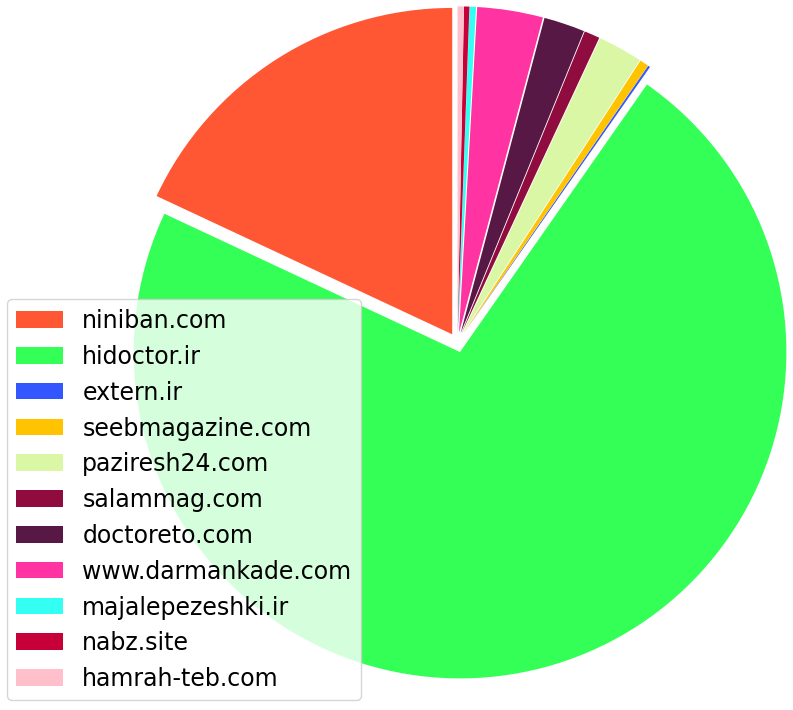
\includegraphics[width=0.4\textwidth]{fig1.png}}
	\caption{Share of articles by magazine}
	\label{fig1}
\end{figure}

\subsection{dataset}
The collection of a real-world doctor-patient question-answering dataset is crucial for enhancing the capabilities of language models in the healthcare domain. Such a dataset allows models to learn valuable information derived from authentic interactions between healthcare providers and patients. By analyzing these real-world exchanges, language models can grasp the nuances of medical terminology, patient concerns, and the context surrounding healthcare inquiries. Furthermore, this dataset equips models with the ability to learn not just the factual content of responses but also the appropriate structure and tone for answering questions. This dual learning process is essential, as it enables the model to generate accurate, empathetic, and contextually relevant responses, ultimately improving patient communication and support in medical environments. In this context, Yang Liu \cite{b6} highlights several real-world doctor-patient question-answering datasets in his survey, and a comparison of these datasets with ours can be found in Table II. In an era where technology increasingly aids healthcare, a robust doctor-patient dataset stands as a foundational element in training models that can effectively contribute to better healthcare delivery.

\begin{table}[ht]
	\centering
	\caption{Comparison of Our dataset with others}
	\begin{tabular}{|l|c|c|c|}  % Using vertical lines for a simple table
		\hline
   name            &language & no. records & collected by \\ \hline
   ChatDoctor 	   &English	 & 100K        & Yunxiang Li et all
   \cite{b10}
    \\ \hline
   CMtMedQA  	   &Chinese	 & 68K        &  Songhua Yang et all
   \cite{b10}
   \\ \hline
   DISC-Med-SFT	   &Chinese	 & 465K       & Zhijie Bao et all   
   \cite{b10}
   \\ \hline
   HuatuoGPT-	   &Chinese	 & 226K        & Hongbo Zhang et all   
   \cite{b10}
    \\ 
   sft-data-v1	   &	     &             & 	\\ \hline
   Huatuo-26M	   &Chinese	 & 26M         & Jianquan Li et all 
   \cite{b10}
   \\ \hline
   MedDialog       &Chinese \&&3.66M       & Guangtao Zeng et all  \\ 
                   &English  &             &   \\ \hline
   Medical Meadow  &English  & 160k        & Tianyu Han et all 
   \cite{b10}
   \\ \hline
   MF3QA           &Persian  & 20k            & us \\ \hline
	\end{tabular}
	\label{tab:model_results_on_mcqa}
\end{table}


In our research, we crawled more than 180,000 question-answer pairs from Persian medical forums, employing both manual and automatic filtering methods to refine the dataset through a laborious cleaning process. This approach is similar to the work done by Yunxiang Li et al. \cite{b6} in their article on the Chat Doctor medical language model, where they extracted data from English medical forums. Notably, Yunxiang Li discarded about half of the question-answer pairs based on the length of the answers, as shorter responses are generally inadequate for training a model and can lead the model to learn to provide brief answers. However, we faced a greater challenge; Persian doctors tend to provide much shorter answers compared to their English counterparts, resulting in the necessity to discard over 80\% of our question-answer records to ensure quality and relevance for our training purposes.

To create our dataset, we utilized patient-doctor interactions from the drhast and niniban platforms for the training split. It is important to note that drhast does not provide all of its doctor-patient interaction records on its site; it only offers access to the last 2,000 records. Additionally, each record is linked to 100 related records, complicating the crawling process. To address this challenge, we treated their data as a graph and performed a breadth-first search, which took about two weeks to extract 120,000 records out of a total of 200,000. For the test set, we used the doctor-yab and isovisit sites, ensuring diversity by translating the KQA question-answering dataset
\cite{b10}
and appending it to our test split. This comprehensive approach not only enriched our dataset but also underscored the importance of real-world doctor-patient interactions in training effective language models.

\section{Training}
\subsection{fine tuning}
We fine-tuned the aya-expanse8b model on 60\% of our corpus, leveraging LoRA
\cite{b13}
method to optimize performance. Specifically, we implemented a rank of 8, an alpha value of 16, and a LoRA dropout rate of 0.05, conducting the fine-tuning for a single epoch. This approach allowed us to effectively adapt the model to our specific dataset while minimizing resource usage, ensuring a balance between efficiency and performance enhancement in our training process.
\subsection{instruction tuning}
In addition to fine-tuning the aya-expanse8b model, we also instruction-tuned the fine-tuned model on our crawled free-form Farsi question-answering (MF3QA) dataset. For this instruction tuning, we employed a LoRA method with a rank of 2, an alpha value of 2, and a LoRA dropout rate of 0.4, conducting the process for a single epoch. This targeted approach allowed us to further enhance the model’s ability to understand and generate responses in the context of Farsi question-answering, optimizing its performance for our specific dataset and improving its overall effectiveness.
\subsection{Carbon Footprint}
During our recent computational experiments, we utilized an A100 PCIe 40/80G hardware setup on the Google Cloud Platform, specifically in the asia-east1 compute region. The hardware was operational for a total of 19 hours, resulting in a carbon footprint of 2.66 kg CO2 equivalent emissions calculated  based on the formula introduced by Wu et all
\cite{b14}
.
\section{Results}
Since there is no publicly available medical Persian language model to compare our results against, and given that only a few small Persian language models exist, we opted to compare our model with a pipeline system that combines an English medical language model with a translator, specifically targeting systems with a total of less than 8 billion parameters, which we define as runnable on home devices. We evaluated our model against two different pipeline configurations to demonstrate that, in addition to their poor grammatical performance, these systems also struggle to effectively encode medical knowledge, as evidenced by their low scores in multiple-choice question-answering datasets. The first configuration involved using MedMobile
\cite{b9}
as the English small medical language model paired with gemma-2b-it
\cite{b15}
as the translator, while the second configuration used MedMobile with Parsinlu
\cite{b16}
\cite{b17}
as the translator. Our comparisons highlighted the limitations of these pipeline systems in both linguistic accuracy and medical comprehension.
\footnote{
	you can see the detailed result at https://github.com/Mehrdadghassabi/Gaokerena
}
\subsection{multiple choice question answering}
In our results section, we address the significant challenge of the lack of available Persian datasets for medical language processing. To overcome this, we translated the medical portion of the Massive Multitask Language Understanding (MMLU)
\cite{b18}
dataset into Persian and supplemented it with data from the Iranian Basic Medical Sciences Entrance Exam(IBMSEE), which we also crawled. Notably,as you can see on Table
\ref{tab:model_results_on_mcqa}
our model achieved remarkable success by surpassing the passing score of the Iranian Basic Medical Sciences Entrance Exam, which stands at 36\%, making it the first Persian small language model to pass this exam. Furthermore, our model demonstrated substantial improvements on the translated MMLU dataset, not only achieving higher average scores but also excelling across most sub-categories, thereby showcasing its effectiveness in understanding and generating medical knowledge in the Persian language.
\begin{table}[ht]
	\centering
	\caption{Results on medical multiple choice question answering}
	\begin{tabular}{|l|c|c|c|c|}  % Using vertical lines for a simple table
		\hline
		\textbf{} & \textbf{Gao-} & \textbf{aya-}
		 & \textbf{MedMobile} & \textbf{MedMobile} \\ 
		 & \textbf{kerena} & \textbf{expanse8b} & + \textbf{gemma2b-it} & \textbf{+ parsinlu} \\
		 & (ours) & (baseline) &  &  \\ \hline
		MMLU- & \textbf{48.14} & 40.74 & 14.07 & 25.18 \\ 
		anatomy(fa) &  &  &  &  \\ \hline
		MMLU- & 46.0 & \textbf{49.0} & 20.0 & 35.0 \\
		medical &  &  &  &  \\ 
		genetics(fa) &  &  &  &  \\ \hline
		MMLU- & 43.93 & \textbf{44.51} & 19.08 & 27.17 \\
		college &  &  &  &  \\
		medicine(fa) &  &  &  &  \\ \hline
		MMLU- & \textbf{55.47} & 52.07 & 27.54 & 31.7 \\
		clinical&  &  &  &  \\
		knowledge(fa)&  &  &  &  \\ \hline
		MMLU- & ? & ? & ? & ? \\
        professional&  &  &  &  \\ 
        medicine(fa)&  &  &  &  \\ \hline
        MMLU- & \textbf{47.22} & 45.14 & 18.75 & 31.25 \\
        college&  &  &  &  \\
        biology(fa)&  &  &  &  \\ \hline
        MMLU(avg) & ? & ? & ? & ? \\ \hline
		IBMSEE & \textbf{38.69} & 34.52 & 24.40 & 32.73 \\ 
        (sept 2023) &  &  &  &  \\  \hline
	\end{tabular}
	\label{tab:model_results_on_mcqa}
\end{table}
\subsection{free form question answering}
\subsubsection{K-QA benchmark}
In this study, we utilized the K-QA dataset introduced by Itay Manes
\cite{b19}
, which consists of expert-generated question-answer pairs, each accompanied by “nice to have” and “must have” lists. Manes proposed two key metrics, Completeness and Factuality, which are essential for evaluating the quality of the question-answer pairs. These metrics, as reformulated by Hyunjae Kim
\cite{b8}
, are defined as follows:  
\[
S_{comp}(r_i,A_i^{\prime}) =  \sum_{a \in A_i^{\prime}} \frac{[r_i \: entails \: a]}{|A_i^{\prime}|}
\]
\[
S_{fact}(r_i,A_i^{\prime}) = 
\begin{cases} 
	0 & \text{if } \exists a \in A_i \: s.t.  \: r_i \: contradicts \: a\\ 
	1 & otherwise
\end{cases}
\]
Manes likened these metrics to traditional precision and recall, leading to the introduction of a new metric, the $F_{1}^{\prime}$ score, analogous to the $F_{1}$ score, defined as: 
\[
F_{1}^{\prime} = \frac{2 \times S_{comp} \times S_{fact}}{S_{comp} + S_{fact}}
\]
In our research, we translated the K-QA dataset into Persian and computed the Completeness and Factuality scores for our model, Gaokerena, as well as for the baseline model,aya-expanse-8b. as you can see in the Table
\ref{tab:model_accuracy_on_ffqa}
the results indicated that Gaokerena slightly outperformed aya-expanse-8b in both the $F_{1}^{\prime}$ score and the Factuality score, demonstrating the effectiveness of our approach.

\begin{table}[ht]
	\centering
	\caption{Results on k-qa benchmark}
	\begin{tabular}{|c|c|c|} % l for left-aligned, c for centered
		\hline
		\textbf{} & \textbf{gaokerena} & \textbf{aya-expanse-8b} \\ 
		\hline
		$S_{comp}$ & 0.7194 & \textbf{0.7322} \\ 
		\hline
		$S_{fact}$ & \textbf{0.4925} & 0.4776 \\ 
		\hline
		$F_{1}^{\prime}$ & \textbf{0.5847} & 0.5781 \\ 
		\hline
	\end{tabular}
	\label{tab:model_accuracy_on_ffqa}
\end{table}

\subsubsection{AI Evaluating AI}
In addition to our K-QA benchmark, we also utilized GPT-4o
\cite{b20}
as an evaluator for free form question answering. We provided the test set from the MF3QA dataset to both aya-expanse-8b and our model. As illustrated in figure
\ref{fig2}
,GPT-4o predominantly preferred the responses generated by our model to the baseline model. This indicates that our model delivers high-quality responses as judged by an advanced language model.

\begin{figure}[htbp]
	\centerline{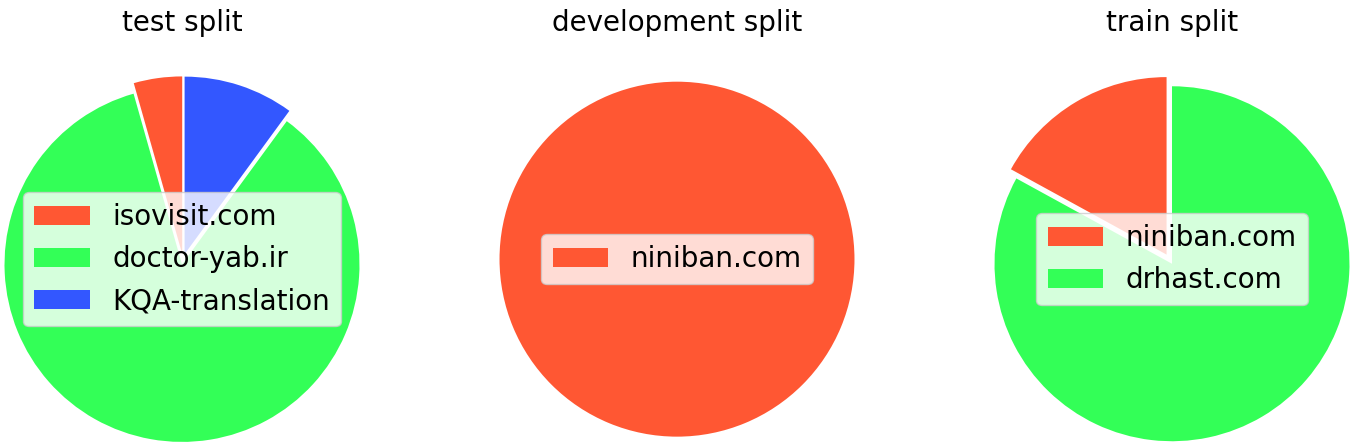
\includegraphics[width=0.4\textwidth]{fig2.png}}
	\caption{GPT-4o choice}
	\label{fig2}
\end{figure}
\section*{Acknowledgment}
We would like to thank Amir Jahani for his help with the data cleaning process.


\begin{thebibliography}{00}
\bibitem{b1} Vaswani, Ashish, et al. "Attention is all you need." Advances in neural information processing systems 30 (2017).
\bibitem{b2} Singhal, Karan, et al. "Toward expert-level medical question answering with large language models." Nature Medicine (2025): 1-8.
\bibitem{b3}
Singhal, Karan, et al. "Large language models encode clinical knowledge." Nature 620.7972 (2023): 172-180.
\bibitem{b4} Taghizadeh, Nasrin, et al. "SINA-BERT: a pre-trained language model for analysis of medical texts in Persian." arXiv preprint arXiv:2104.07613 (2021).
\bibitem{b5} Dang, John, et al. "Aya expanse: Combining research breakthroughs for a new multilingual frontier." arXiv preprint arXiv:2412.04261 (2024).
\bibitem{b6} Li, Yunxiang, et al. "Chatdoctor: A medical chat model fine-tuned on a large language model meta-ai (llama) using medical domain knowledge." Cureus 15.6 (2023).
\bibitem{b7} Touvron, Hugo, et al. "Llama: Open and efficient foundation language models." arXiv preprint arXiv:2302.13971 (2023).
\bibitem{b8} Kim, Hyunjae, et al. "Small language models learn enhanced reasoning skills from medical textbooks." arXiv preprint arXiv:2404.00376 (2024).
\bibitem{b9} Vishwanath, Krithik, et al. "MedMobile: A mobile-sized language model with expert-level clinical capabilities." arXiv preprint arXiv:2410.09019 (2024).
\bibitem{b10} Abdin, Marah, et al. "Phi-3 technical report: A highly capable language model locally on your phone." arXiv preprint arXiv:2404.14219 (2024).
\bibitem{b11} Team, Gemma, et al. "Gemma: Open models based on gemini research and technology." arXiv preprint arXiv:2403.08295 (2024).
\bibitem{b12} Rostami, Pedram, Ali Salemi, and Mohammad Javad Dousti. "Persianmind: A cross-lingual persian-english large language model." arXiv preprint arXiv:2401.06466 (2024).
\bibitem{b13} Hu, Edward J., et al. "Lora: Low-rank adaptation of large language models." ICLR 1.2 (2022): 3.
\bibitem{b14} Lacoste, Alexandre, et al. "Quantifying the carbon emissions of machine learning." arXiv preprint arXiv:1910.09700 (2019).
\bibitem{b15} Team, Gemma, et al. "Gemma 2: Improving open language models at a practical size, 2024." URL https://arxiv. org/abs/2408.00118 1.3 (2024).
\bibitem{b16} Khashabi, Daniel, et al. "Parsinlu: a suite of language understanding challenges for persian." Transactions of the Association for Computational Linguistics 9 (2021): 1147-1162.
\bibitem{b17} Kashefi, Omid. "MIZAN: a large persian-english parallel corpus." arXiv preprint arXiv:1801.02107 (2018).
\bibitem{b18} Hendrycks, Dan, et al. "Measuring massive multitask language understanding." arXiv preprint arXiv:2009.03300 (2020).
\bibitem{b19} Manes, Itay, et al. "K-qa: A real-world medical q\&a benchmark." arXiv preprint arXiv:2401.14493 (2024).
\bibitem{b20} Hurst, Aaron, et al. "Gpt-4o system card." arXiv preprint arXiv:2410.21276 (2024).
\end{thebibliography}


\end{document}
